\section{PI szabályzó tervezése pólus-zérus kiejtéssel}

%{{{ P és I paraméterek számításaP és I paraméterek számítása
\subsection{P és I paraméterek számítása}

\Aref{fig:pi-hatasvazlat}. ábra mutatja a rendszerünket, ahol a $ \fn{W}_\text{c} $ szabályzó átviteli függvénye
\begin{equation}
	\fn{W}_\text{c} = P\frac{1+sT_\text{I}}{sT_\text{I}}
\end{equation}
alakú.
$T_\text{I}$-vel a motor legnagyobb időállandóját ejtjük ki, tehát ezt válasszuk $T_\text{I}=T_1=0,0145$ s értékűre,
az első házi feladatban kiszámoltak alapján.

Az előrevezető ág átviteli függvénye ekkor leegyszerűsödik:
\begin{equation}
	\fn{W}_\text{x} = \frac{A}{\bcancel{(1+T_1s)}(1+T_2s)}P\frac{\bcancel{1+sT_\text{I} }}{sT_\text{I}}
	= \frac{AP}{T_\text{1}}\frac{1}{s(1+sT_2)},
\end{equation}
ahol $T_1$ és $T_2$ a szabályozott szakasz időállandója, $A$ az erősítése.

Most írjuk fel a fáziskésést az $s=j\omega$ helyettesítéssel.
\begin{equation}
	\varphi(\omega) = \underbrace{-\frac{\pi}{2}}_\text{integráló tag miatt} - \underbrace{\operatorname{arctg}(T_2\omega)}_\text{kisebbik időállandó}.
\end{equation}
A megadott fázistartalék $\varphi_\text{t} = \vartheta_1=60^\circ$. A következő egyenlet megoldása adja a vágási
körfrekvenciát:
\begin{equation}
	\varphi_\text{t} = \varphi(\omega_\text{c}) +\pi \,\Rightarrow\, \omega_\text{c} = 4176,1~\frac{\text{rad}}{\text{s}}
\end{equation}
Ha $\omega_\text{c}$ a vágási körfrekvencia, definíció szerint $\abs{\fn{W}_\text{x}(\omega_\text{c})} = 1$.
Ez alapján $ P = 4,0709$.

A MATLAB-ban található \verb|margin| függvény segítségével ellenőrizzük a számolást, amit \aref{fig:1a_margin}. ábra igazol.
\begin{figure}[H]
	\centering
	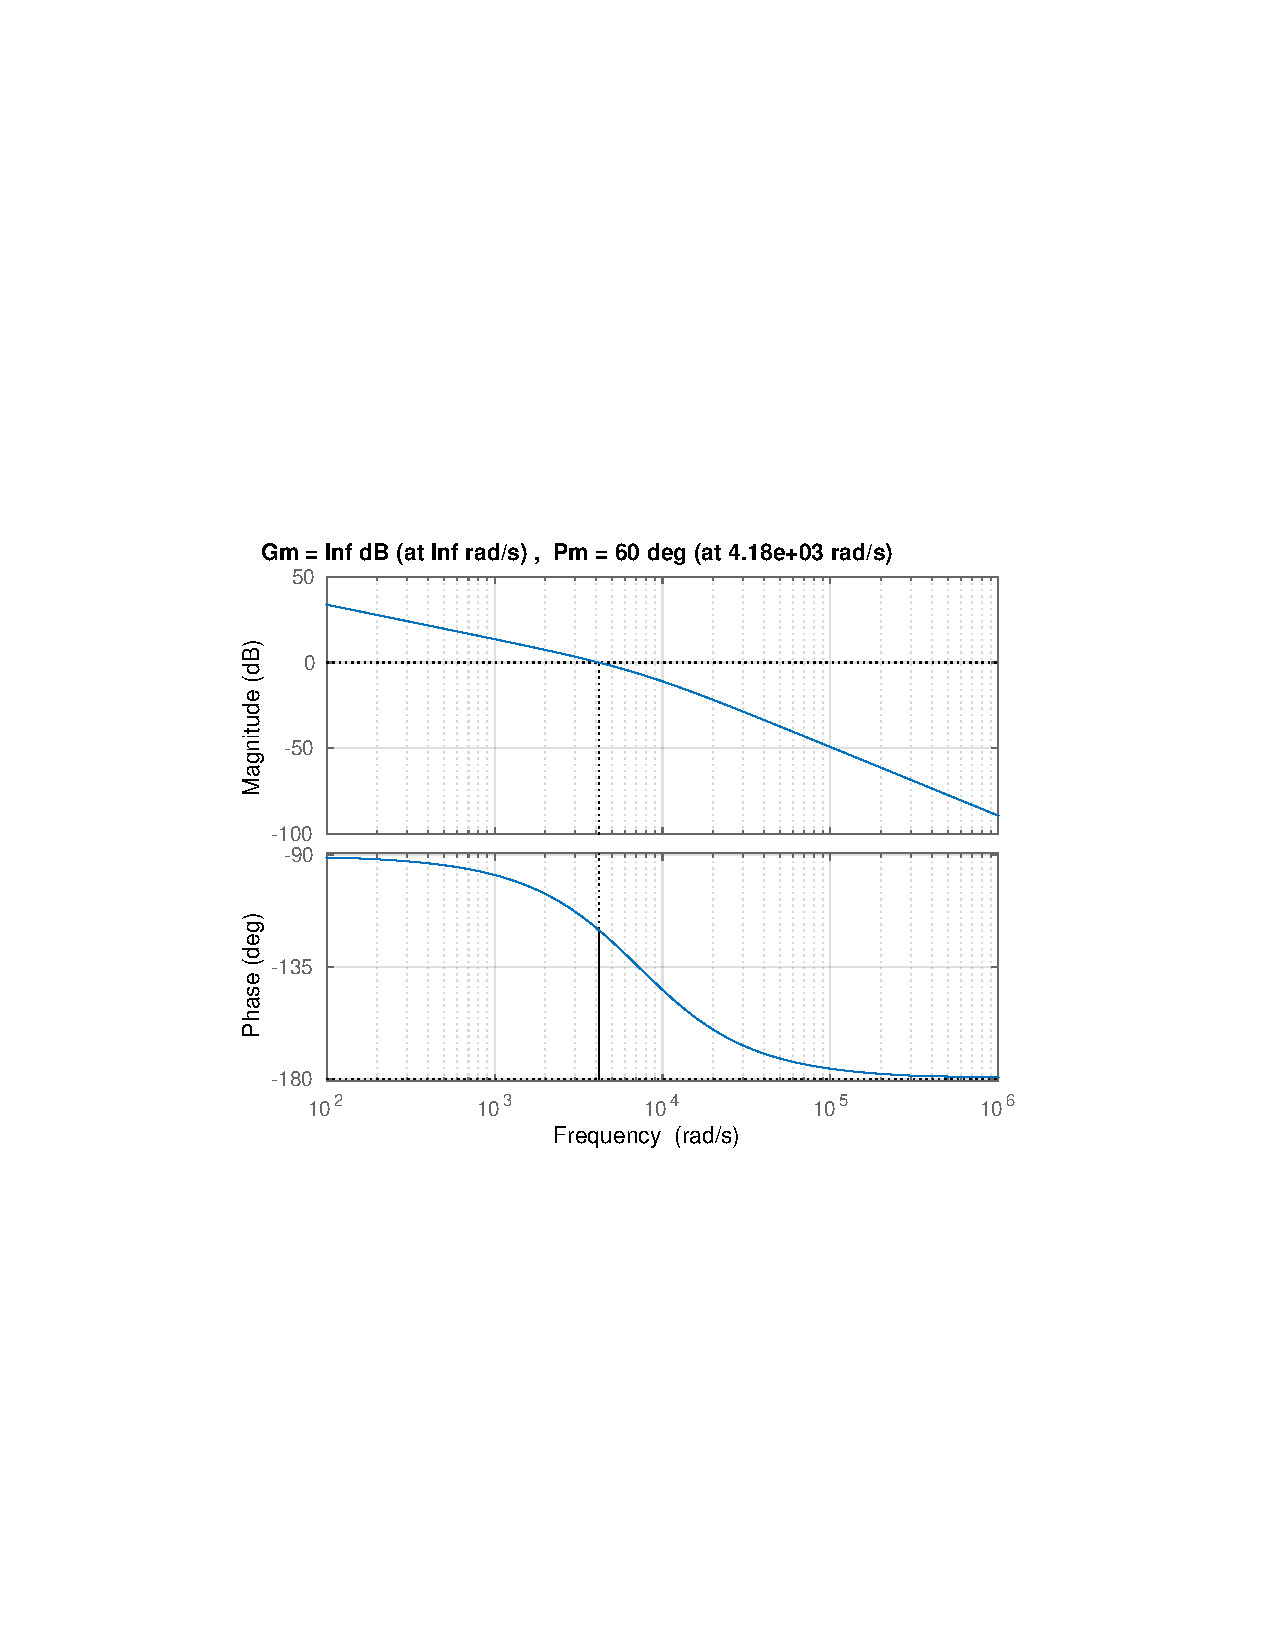
\includegraphics[width=.8\textwidth, trim=100 240 80 252, clip]{1a_margin}
	\caption{Szabályozott rendszer Bode-diagramja}
	\label{fig:1a_margin}
\end{figure}

%}}}

%{{{ Egységugrás válasz
\subsection{Egységugrás válasz}

Az előrevezető ág $\fn{W}_\text{x}$, a zárt kör átviteli függvénye ebből
\begin{equation}
	\fn{W}_\text{cl} = \frac{\fn{W}_\text{x}}{1+\fn{W}_\text{x}},
\end{equation}
mivel a visszacsatoló ágban $\fn{W}_\text{fb}=1$.
Ezt meg kell szorozni az $\omega_\text{ref} = 4430$ rpm $ = 705.0564~\frac{\text{rad}}{\text{s}} $ referencia szögsebességgel.

A PI-szabályozott rendszer egységugrás-válaszát a MATLAB-os \verb|step| függvény adja meg.
\begin{figure}[H]
	\centering
	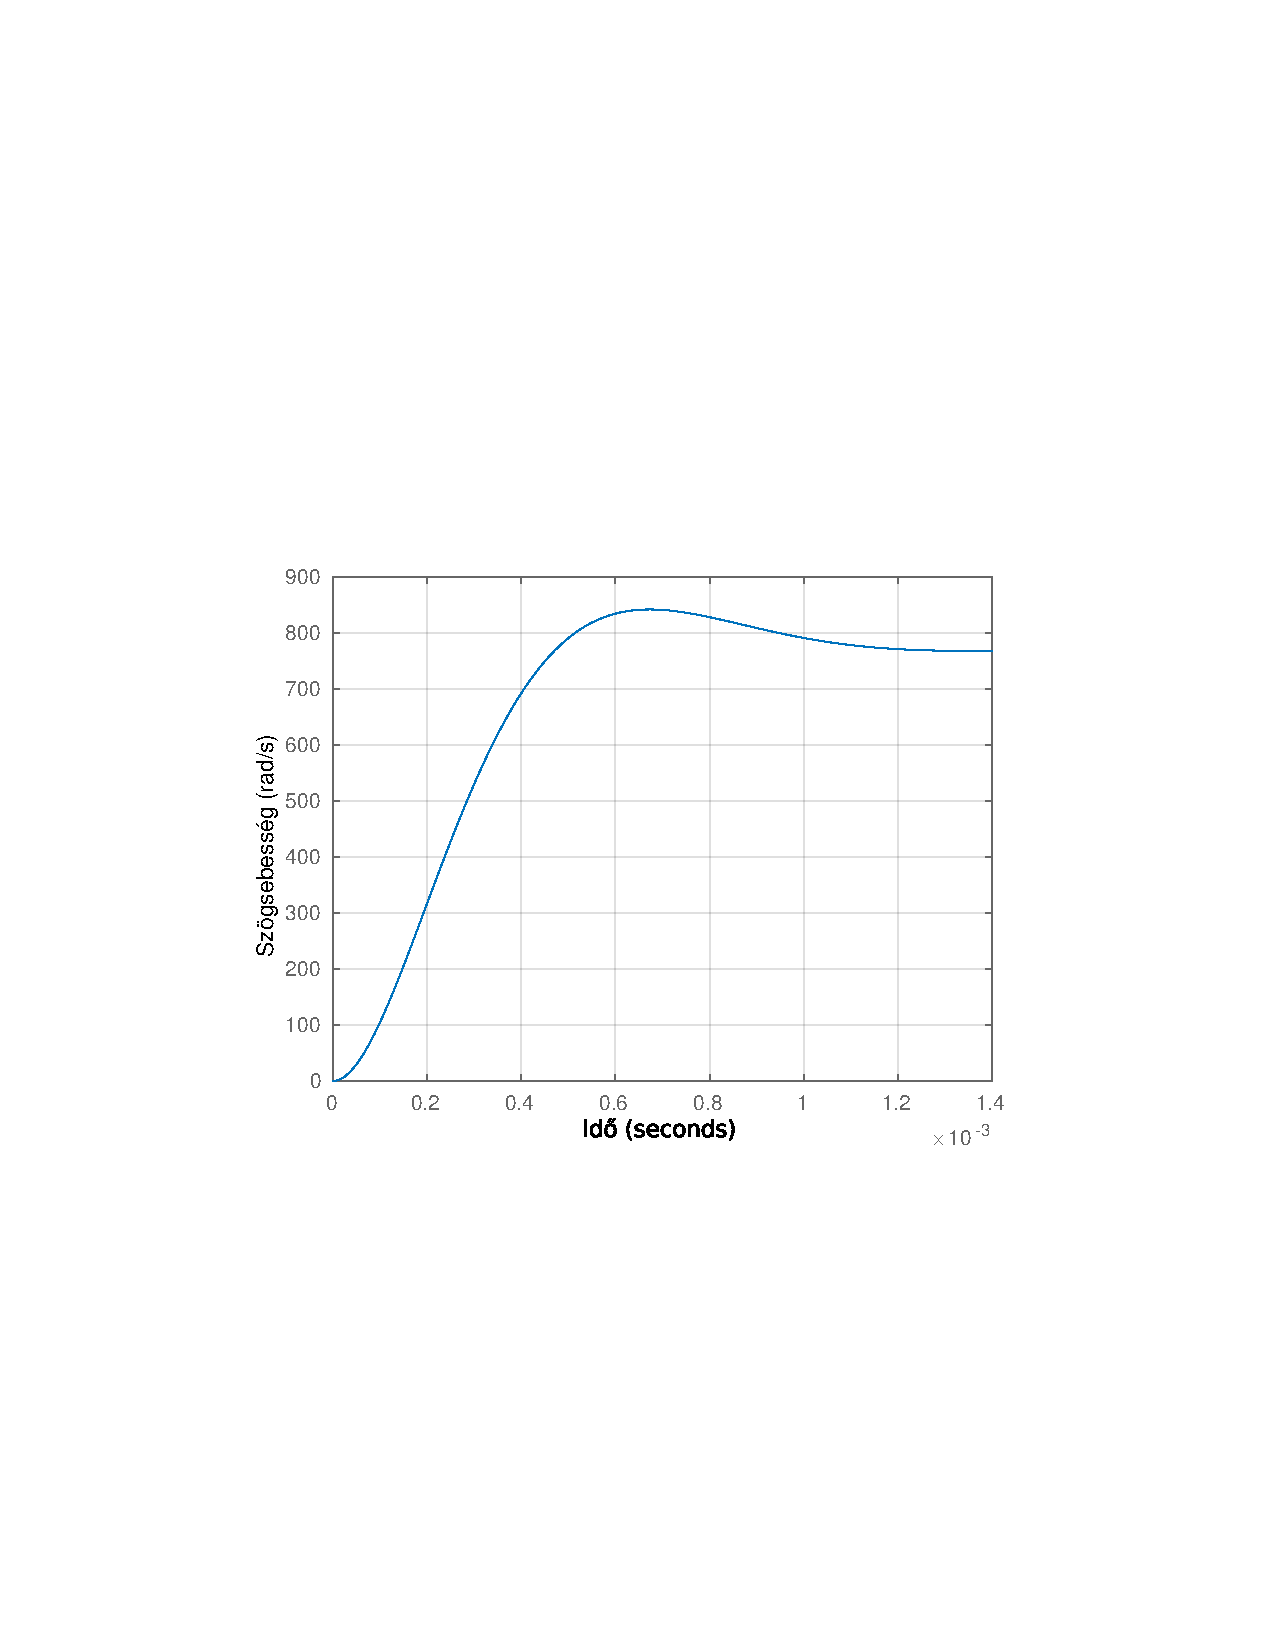
\includegraphics[width=.8\textwidth, trim=100 240 80 252, clip]{1b_step}
	\caption{PI egységugrás-válasz}
	\label{fig:1b_step}
\end{figure}

%}}}

%{{{ Állandósult szögsebesség
\subsection{Állandósult szögsebesség}

A bemenet legyen $\fn{X} = \frac{\omega_\text{ref}}{s}$, a rendszer válasz $\fn{Y} = \fn{W}_\text{cl}\fn{X}$.
A végérték-tétel alapján $\omega_\infty = \lim\limits_{s\rightarrow 0}s\fn{Y} = 705,0564$.

%}}}
